\documentclass{article}
\usepackage{amsmath,amssymb}
\usepackage{graphicx}
\usepackage{bm}
\usepackage[numbers]{natbib}
\usepackage{color}

\title{The binary liquid model for gravity-driven microchannel simulations}
\date{\today}


\begin{document}

\maketitle

\begin{abstract}
The motion towards exploration of nano- and microscale phenomena brings new
challenges to simulation tools. The continuous physics approach is limited on
those scales, therefore such methods as Molecular Dynamics (MD) or Lattice
Boltzmann Method (LBM) become appropriate. This work has aim to
reproduce the gravity driven microchannel flow of free surface liquid with the
help of the binary liquid lattice Boltzmann method. In the low capillary number
$Ca$ region the flow is thoroughly described by Bretherton \cite{bretherton},
where the deposition film thickness is proportional to $Ca^{2/3}$. The binary
liquid model is continuous interface multiphase model. Therefore, the issue of
how to properly resolve the interface to obtain proper correlations holds. In
the work we address the binary liquid parameters, as mobility $M$, surface
tension parameter $k$, the free energy constant $A$, grid resolution, to
properly simulate microchannel flow. The work is valuable for industry and
researchers willing to simulate Bretherton phenomena.
\end{abstract}


\section{Introduction}
Taylor/Bretherton \cite{bretherton} flow describes flow of long bubbles in
microchannels. It was found that the front meniscus film width is proportional
to $Ca^{2/3}$ for Capillary numbers less than $0.003$. While there are number
of works which simulate the Bretherton problem with the boundary value method
\cite{ingham-plates,heil-bretherton}, the simulation of Bretherton problem is of
difficulty for diffusion interface methods, where the interface is spread over
the few grid nodes. In this case the question of proper film width resolution
arises. While the discontinuous interface models are good to simulate
non-complicated geometries phenomena, the continuous interface methods are more
flexible to resolve problem evolving coalescence or droplet breakup. This work
concentrates on the resolving parameters range of the binary liquid lattice
Boltzmann method to validate it across the Bretherton problem. 

Lattice Boltzmann method has emerged as successful method to simulate various
phenomena as hydrodynamics \cite{yu}, thermal-flows
\cite{karlin-minimalmodels}, micro-flows \cite{ansumali-small-knudsen},
ferrofluids \cite{kuzmin-aniso}, and multiphase flows
\cite{swift,Shan-chen:extended}. Based on kinetic nature and as a particle
method LBM tackles relatively easy complex geometries and the incorporation of
physics phenomena on the microscopic level, as multiphase models. Most
multiphase lattice Boltzmann models \cite{swift, Shan-chen:extended} resolve
the interface in the continuous way. Such representation as it was pointed out
brings issues with the film thickness resolution versus the interface
resolution. In other words, when it comes to the resolution of the film
thickness the diffusion interface should be resolved in such way as to have
negligible effect on physics in the film. 

This work examines the binary liquids free-energy LBM model \cite{swift}. The
model simulates binary liquids within the assumption of the uniform overall
density. Therefore, the question of how to simulate the Bretherton problem
where two phases are completely of different densities (liquid and gas) is of
interest. However, the motion of a liquid slug and a bubble in a capillary is
governed by the capillary number. Therefore, the viscosities ratio not the
densities ratio is the critical parameter. 

The goal of this paper is to give the answer as to how to choose related to the
binary liquid model parameters, viscosities ratio and grid
resolution to obtain the Bretherton/Taylor problem film thickness for the
diffusion interface model. The paper is organized as follows. We briefly
explain the binary liquid lattice Boltzmann model and summarize literature
review for the Bretherton problem. Then the parameters involved in the
simulation are examined and presented in the results section. The paper is
concluded with main findings.

\section{Bretherton bubble flow}
Bretherton in his significant work \cite{bretherton} studied a long bubble
moving in a tube filled with liquid. It was found that the deposition film is
proportional to $Ca^{2/3}$ in the range of small capillary numbers. Later on
it was figured \cite{wong-films,wong-pressure} that the film deposition
proportinal to $Ca^{2/3}$ only near the front meniscus and the film width is
variated through the bubble length for not infinite bubbles. Numerical
simulations \cite{giavedoni-numerical} and experimental studies
\cite{kreutzer-pressure-drop} show as well the deviation of rule $Ca^{2/3}$ for
capillary numbers more than $0.003$ and Reynolds number dependance. To be able
to predict consistently the flow pattern for capillaries in different range of
the parameters researchers validate their codes with the small capillary
numbers Bretherton problem.  

There are a number of the numerical methods which
were used for the Taylor/Bretherton flow
simulation. \citet{vanbaten-circular} studied the mass transfer and film
thickness for rising bubbles in a circular capillar.
\citet{kreutzer-pressure-drop} performed numerical simulation by the
finite volume method the circular capillary for the number of different
Reynolds and capillary numbers. \citeauthor{wong-films} in
\cite{wong-films,wong-pressure} studied three-dimensional bubbles in the
polygonal capillaries and showed the derivations of different shapes in the
slug crossections and menisci appearance.
\citet{heil-bretherton,ingham-plates} studied the air finger propagation to
the two-dimensional channel for the range of Reynolds numbers and capillary
numbers. \citet{giavedoni-numerical} performed crossvalidation of the
finite element solution developed by them with the already published results
across the different capillary numbers. The solution is available for circular
and planar cases. 

While the applicability of other methods are well established for the
simulation of the Bretherton/Taylor problem, the lattice Boltzmann
applicability and thorough parameters study to the best authors' knowledge is
not yet done. Especially that concerns the diffuse interface multiphase
models, where one needs to resolve the film accordingly. One should acknowledge
the works of
\citet{pagonabarraga-fingers} on meniscus in thin films for the fingering
phenomena. \citet{sehgal-microchannel} performed the lattice Boltzmann
simulations of two-dimensional channel flow for larger capillary numbers where
the authors found the discrepancies with the classical Bretherton theory having
limitations to the low capillary numbers regime \cite{giavedoni-numerical}.

While to resolve interface on a fine level for capillary numbers less than
$0.003$ is computationally extensive even for a two-dimensional case. For
instance for capillary number $0.01$ to properly resolve the interface one
needs around 22 GB memory requirement. Therefore, this work is based on the
comparison with the already established results which were in their case
validated over the Bretherton bubble flow. The work presents recipes for the
initialization and the optimal parameter range for the binary liquid LBM model,
which is described in the next section. 

\section{Lattice Botlzmann binary liquid model}
The lattice Boltzmann equation operates on the rectangular grid representing the
physical domain. It utilizes the
probability distribution functions containing the information about the
macroscopic variables, such as density,
momentum. LBE consists from two parts: local collision and propagation operated
from one node to another in the certain
direction specified by the velocity set.  The lattice Boltzmann implementation
in a standard view representing the
collision and propagation steps:
\begin{equation}
\label{standard:implementation}
\begin{aligned}
&f_i^{*}(\bm{x},t)=\omega f_i^{eq}(\bm{x},t)-(1-\omega) f_i(\bm{x},t) +
F_i,&&\text{ collision step}\\
&f_i(\bm{x}+\bm{c_i},t+1)=f_i^{*}(\bm{x},t),&&\text{ propagation step}, 
\end{aligned}
\end{equation}
where $F_i$ is the external force population. The binary liquid LBM model is
based on the free-energy functional \cite{swift,landau} and operates with two
sets of populations one to track pressure and velocities fields, another one is
for the phase field. The model to be utilized is two-dimensional nine-velocity
D2Q9 model.

In terms of D2Q9 the equilibrium populations are as \cite{pooley-contact}:
\begin{equation}
\begin{aligned}
&f_i^{eq}=w_i 
\biggl(3
p_0 - k \phi \Delta \phi
+\frac{u_{\alpha}c_{i\alpha}}{c_s^2}+\frac{Q_{i\alpha\beta}u_{\alpha } u_ {
\beta}}{2 c_s^4}\biggr), i=1\div8\\
&f_0^{eq}=\rho-\sum_{i\neq0}{f_i^{eq}}\\
&g_i^{eq}=w_i(\Gamma \mu + \frac{\phi c_{i\alpha} u_{i\alpha}}{c_s^2}+\phi^m
\frac{Q_{i\alpha\beta}u_{\alpha}u_{\beta}}{2 c_s^4}), i=1\div8 \\
&g_0^{eq}=\phi-\sum_{i\neq0}{g_i^{eq}}\quad,
\end{aligned}
\end{equation}
where $\Gamma$ is the mobility parameter; chemical potential
$\mu=-A\phi+A\phi^3-k\Delta\phi$; $k$ is related to the surface
tension; $A$ is the parameter of the free-energy model; bulk pressure
$p_0=c_s^2 \rho +A (-0.5 \phi^2+0.75 \phi^4)$. D2Q9 related parameters are
$w_i=\left\{\frac{4}{9},\frac{1}{9},\frac{1}{9},\frac{1}{9},\frac{1}{9},
\frac{1}{36},\frac{1}{36},\frac{1}{36},\frac{1}{36}\right\}$, and
$Q_{i\alpha\beta}=c_{i\alpha} c_{i\beta} - c_s^2 \delta_{\alpha\beta}$ with
the sound speed parameter $c_s^2=\dfrac{1}{3}$. Weights related to the
inclusion of the surface tension coefficient are as follows:
$w^{xx}_{1-2}=w^{yy}_{3-4}=1/3$, $w^{xx}_{3-4}=w^{yy}_{1-2}=-1/6$,
$w^{xx}_{5-8}=w^{yy}_{5-8}=-1/24$, $w^{xy}_{1-4}=0$, $w^{xy}_{5-6}=1/4$ and
$w^{xy}_{7-8}=-1/4$. Note that the system restores the macroscopic
equations as:
\begin{equation}
\begin{aligned}
&\partial_t \rho+ \partial_{\alpha} \rho u_{\alpha}=0\\
&\rho\left(\partial_t+u_{\beta}\partial_{\beta}\right) u_{\alpha}=
-\partial_{\alpha}P_{\alpha \beta} +
\nu\partial_{\beta}\left(\partial_{\alpha}u_{\beta}+\partial_{\beta} u_{\alpha}
+ \frac{1}{3}\partial_{\gamma} u_{\gamma} \delta_{\alpha\beta}\right)\\
&\partial_t \phi + \partial_{\alpha} \phi u_{\alpha}=M \Delta \mu,
\end{aligned}
\label{binary:fluid:system}
\end{equation}
where the viscosity $\nu=c_s^2 (\tau-1/2)$ and mobility parameter
$M=\Gamma(\tau_{\phi}-1/2)$. The system allows the separation of the liquid
phase with $\phi=1$ and so-called gas phase with $\phi=-1$. Note that the
spatial variation of the relaxation parameter depends on the relaxation
parameter of $\tau_{gas}$ and $\tau_{liq}$ linearly as
$\tau=\tau_{gas}+\frac{\phi+1}{2}\tau_{liq}$. Note that the surface tension in
the framework of binary liquid model as $\sqrt{8 k A}{9}$.

\section{Lattice Botlzmann benchmark}
To properly simulate and to compare simulations results with the already
performed simulations one needs to design a numerical benchmark by addressing
the following challenges for the lattice Boltzmann method:
\begin{itemize}
 \item The diffusive interface nature of the multiphase model should not
influence the film width results. This is obviously achieved only for certain
resolutions of the diffuse interface in comparison with the film width.
 \item The spurious currents arising from the surface tension discretization
can influence the mass transfer in the thin film therefore comprimising the
overall solution. Therefore the bubble should be long enough to decrease the
influence of the spurious currents.
 \item The wettability coefficient which is in principle can control the
dynamic angle and menisci appearance \cite{pagonabarraga-finger} should not
influence on the overall solution.
 \item The free-energy model examined in the work is one density/different
viscosities model. Classical Bretherton problem is the free-interface problem
where the film thickness is established by itself. The viscosities ratio should
be large as it is indicated in \cite{pagonabarraga-fingers}, however no studies
address this issue.
  \item The Bretherton problem addresses the bubbles flow driven by pressure
difference but not body force. However, it's relatively difficult to impose the
pressure difference in the framework of the binary liquid model because two
boundary conditions with the associated gradients and laplacians are required.
The pressure boundary conditions for the binary liquid model are currently
under development. Preliminary results show that the differences between
pressure difference flows and body force driven flows are small for the film
deposition thickness, the interest of this study. Thus, the work's focus is at
the body force driven flows because of the better simulation stability and
realization along with the periodic boundary conditions.
 \item Most simulations are done across the circular shape of channel,
which is quite difficult to address in terms of lattice Boltzmann free energy
framework where one needs to calculate the laplacians near the boundaries.
Although one can apply certain finite difference stencils
\cite{arnold-boundary,hunt-boundary} developed for the curved boundaries
however the analysis of error which can be addressed to the boundary conditions
treatment becomes an issue. Therefore the benchmark is for an axis-symmetric
case. 
\end{itemize}
Given all the concerns and challenges the suggested Lattice Boltzmann framework
is the two-dimensional flow driven by a body force. However, the analytical
solution to this problem, to the best authors' knowledge, is not yet known.
Though some authors \cite{sehgal-microchannel} use the gravity driven model to
validate the Bretherton film thickness, the latter should be used with caution
since the velocity of the bubble is different from the fluid velocity and a
bubble shape
is different in front and rear menisci. \citet{wong-films} indicated that the
film width for polygonal capillaries
changes from $Ca^{1/2}$ on distances $x\propto Ca^{-1}$ to $Ca^{2/3}$ for
distances $x \gg Ca^{-1}$. Therefore, for a bubble to have a formed shape in
the  front meniscus we picked up the bubble length as $5$ channel heights. The
channel length is taken to minimize the influence of one bubble on another,
because of the periodicity of boundary conditions. For the simulations the
channel length is taken as $3$ bubble lenghts giving all together $15$ channel
heights. Figure \ref{fig:benchmark:sketch} represents the benchmark sketch.
\begin{figure}
%\includegraphics[width=0.97\textwidth]{}
\caption{{\color{red} Ask Sasha to help here. The benchmark sketch.}
\label{fig:benchmark:sketch}}
\end{figure}


\section{Results}
\subsection{The nondimensionalization and initialization procedure}
This section is to introduce the procedure of nondimensionalization and
initialization techniques to be able to predict parameters necessary for
simulation. The capillary number governs the interface thickness and defined as:
\begin{equation}
Ca=\frac{U_{bubble} \mu_{liq}}{\gamma},
\end{equation}
where $\mu_{liq}$ is the liquid viscosity, $\gamma$ is the surface tension. The
bubble velocity $U_{bubble}$ is taken in the center of the bubble where the film
thickness is examined. 
While parameters as $\mu_{liq}$, $\gamma$ and capillary number $Ca$ are given
or defined through the model parameters, the velocity $U_{bubble}$ is not
defined. In the simulation we approximately match the velocity with the
Poiseuille profile center velocit, which is given by the equation:
\begin{equation}
\begin{aligned}
U_{bubble} \approx U_{liq}=\frac{H^2}{8
\mu_{liq}}\frac{\mathrm{d}P}{\mathrm{d}x}\\
U_{bubble}\approx
\frac{{N_y}^2}{\frac{8}{6}(\tau_{liq}-\frac{1}{2})}\frac{\mathrm{d}P}{\mathrm{d}
x } ,
\end{aligned}
\end{equation}
By taking the Poiseuille profile one can estimate the body force through the
capillary number and grid resolution:
\begin{equation}
\label{poiseuille:velocity:center}
\begin{aligned}
&\frac{\mathrm{d}P}{\mathrm{d}x}=\frac{8}{{N_y}^2}\gamma Ca.
\end{aligned}
\end{equation}
In reality we iterate the body force value
until the desired velocity and the capillary number as well are achieved. 

After one resolves necessary parameters to run a simulation, one needs to
initialize the macroscopic fields and populations.
The velocity is initialized with $0$ everywhere. Populations are initialized
with the equilbrium values for the binary liquid model including all the phase
gradients and laplacians. The liquid phase is initialized with $1$ and the
gas phase is initialized with $-1$. Though the initialization film thickness
is not involved in the final result for the front meniscus, Fig.
\ref{fig:different:initialization:widths}, we keep the initialized film
thickness as close as possible to the already obtained numerical film
thicknesses \cite{giavedoni-numerical}. Otherwise, the region where the
Bretherton phenomena occurs is dillute, which is obviously seen for the
simulation initialized with the film thickness as $Ny-28$ {\color{red} Michal,
can you please prepare the simulations with the different initialization. Or
just delete different thicknesses initialization}.
\begin{figure}
\includegraphics*[bb=18 350 594 450,width=0.97\textwidth]
{Figures/force_width_6.eps}
\includegraphics*[bb=18 350 594 450,
width=0.97\textwidth]{Figures/force_width_10.eps}
\includegraphics*[bb=18 350 594 450,
width=0.97\textwidth]{Figures/force_width_14.eps}
\caption{\color{red} The phase plots for different bubble widths as
$Ny-12$,$Ny-20$ and
$Ny-28$. Michal, could you please prepare nice pictures for
simulations. Indicate as well the
grid and time steps\label{fig:different:initialization:widths}}
\end{figure}

Here are two different examples presented that can quantitatively show the
initialization procedure for quite different capillary numbers. In these
examples we use $k=0.04$ and $A=0.04$ as optimal binary liquid model parameters.
That explicitly implies the surface tension to be $\sqrt{\frac{8 k
A}{9}}=0.0377$ and the characteristic length of the interface
$5\sqrt{\frac{k}{A}}=5$ lattice boltzmann units. For the sake of simplicity and
stability the relaxations parameter for liquid and gas phases are taken as
$\tau_{liq}=2.5$ and $\tau_{gas}=0.7$. That gives the gas-liquid viscosity ratio
as $10$.  
\begin{description}
 \item[I \bm{$Ca=0.005$}]
  The film width for such small Capillary numbers \cite{bretherton} is
given by equation:
  \begin{equation}
  \frac{h_{\infty}}{H}=1.3375 Ca^{2/3}=0.03899,
  \end{equation}
  where we assume that $2 H$ or $Ny$ in lattice units is the channel width.
Therefore one needs to resolve the interface which is around $2$ percent of
  whole channel width with for instance $8$ lattice units, where $5$ lattice
units occupies the interface width for given. Note that the interface occupies
$62.5$ percent of the interface.  Therefore the channel
  width is $400$ lattice units. We take the bubble length as $5$ channel widths
  and the distance between bubble is as $2$ bubble lengths. It gives the
grid size as $400\mathrm{x}6000$. In terms of computer memory
requirement the calculations with the double precision accuracy demand:
\begin{equation}
\begin{aligned}
&2\text{ set of populations }\mathrm{x}\,\, 8\,\, \text{bytes per population
}\mathrm{x}\,\, 9 \text{ number of
populations}\\
&\mathrm{x}\,400\,\mathrm{x}\,6000\approx 345 \mathrm{MB}. 
\end{aligned}
\end{equation}
Even with this naive assumption for the $50$ percent resolution of the film
widht in comparison with the interface width, one can get the memory
requirement as $345 MB$. 

After resolving the interface one can  calculate the
  velocity from the capillary number as:
  \begin{equation}
  U_{bubble}=0.005 \frac{\gamma}{\mu_{slug}}=0.005
\frac{0.0377}{0.66666}=2.82\,10^{-4},
  \end{equation}
  where $\mu_{slug}=1/3 (2.5-0.5)=0.6666$.
  This velocity implies the following pressure gradient calculated from the
  Poisuielle flow solution:
  \begin{equation}
  \begin{aligned}
  &U_{bubble}=\frac{H^2}{8\mu} \frac{\mathrm{d}P}{\mathrm{d}x}=\frac{Ny^2}{8/3
  (\tau_{liq}-1/2)}\frac{\mathrm{d}P}{\mathrm{d}x}\\
  &\frac{\mathrm{d}P}{\mathrm{d}x}=\frac{8}{Ny^2}\gamma Ca
  \end{aligned}
  \end{equation}
  Therefore the pressure gradient established is the following:
  \begin{equation}
  \begin{aligned}
  \frac{\mathrm{d}P}{\mathrm{d}x}=9.42\, 10^{-9}.
  \end{aligned}
  \end{equation}
  Note that in the case of large grids  height resolution is directly
involved in	
the physical time step as:
\begin{equation}
\Delta t =\frac{U_{LBM}}{U_{phys}} \Delta x ,
\end{equation}
where for example the real velocities in the physical world can reach
approximately $1$ m/s and physical channel height upto $1$ mm. In this case one
can easily approximate the physical time step:
\begin{equation}
\Delta t = 7.05 \, 10^{-10} \,\mathrm{s}
\end{equation}
which is a small time step. The typical simulation needs approximately
{\color{red} $100,000$} time steps to come to the steady state solution.

 \item[II $\bm{Ca=0.05}$] 
   The parameters in the previous subsection imply very long
simulations. Bretherton delivered his solution for the range of Capillary number
less than
  $0.005$. However, a lot of simulations devoted to the Bretherton/Taylor
flow
  simulated and extended it in the range of Capillary numbers greater than
$0.005$
  and for different Reynolds numbers. One can refer to figures
  \ref{fig:giavedoni:planar} and \ref{fig:heil:planar} taken from citations
  \cite{giavedoni-numerical,heil-bretherton} which crossvalidated their
  simulations with Bretherton and each other. Even though LBM can simulate the
flows with small capillary numbers, i.e. less than $0.005$, but waiting time
for the simulation to be accomplished is relatively long. Therefore, we focus
our work on the simulations of \citet{giavedoni-numerical} which crossvalidated
results not only for small capillary numbers but for large capillary numbers as
well. As far as the work intention is
  to show proper physics behavior the moderate parameters are
taken which
  can be easily and fast validated on a computer. 
  One can see from the Fig. \ref{fig:heil:planar} that the width for the
  Capillary number equal to $0.05$ ranges from $0.12$ to $0.15$ while Reynolds
  number ranges from $0$ to $300$. This capillary number has moderate film
widths
  to be resolved with certain accuracy. 

  The film width for such small Capillary numbers is taken from
  \ref{fig:heil:planar} for Reynolds number $40$ equals to $0.12$. We want to
  resolve $6\%$ of whole channel width with $12$ lattice units, where $5$
lattice units are related to the interface resolution.  Therefore the channel
  width is $200$ lattice units. We take the bubble length as $5$ channel widths
  and the distance between slugs we take as $2$ bubble lengths. That gives
the grid size as $200\mathrm{x}3000$. The velocity can be
calculated from the Capillary number as:
  \begin{equation}
  U_{bubble}=0.05 \frac{\gamma}{\mu_{liq}}=0.05 \frac{0.037712}{0.6666}=2.82\,
  10^{-3}.
  \end{equation}
  The velocity implies the following pressure gradient calculated from the
  Poisuielle flow solution:
  \begin{equation}
  \begin{aligned}
  &\frac{\mathrm{d}P}{\mathrm{d}x}=\frac{8}{Ny^2}\gamma Ca=3.77\,10^{-7}.
  \end{aligned}
  \end{equation}
  The initialization approach is to take values from the already performed
numerical simulation and to calculate the grid numbers from them matching the
body force gradient through the solution of Poiseuille flow.   

\end{description}
\begin{figure}
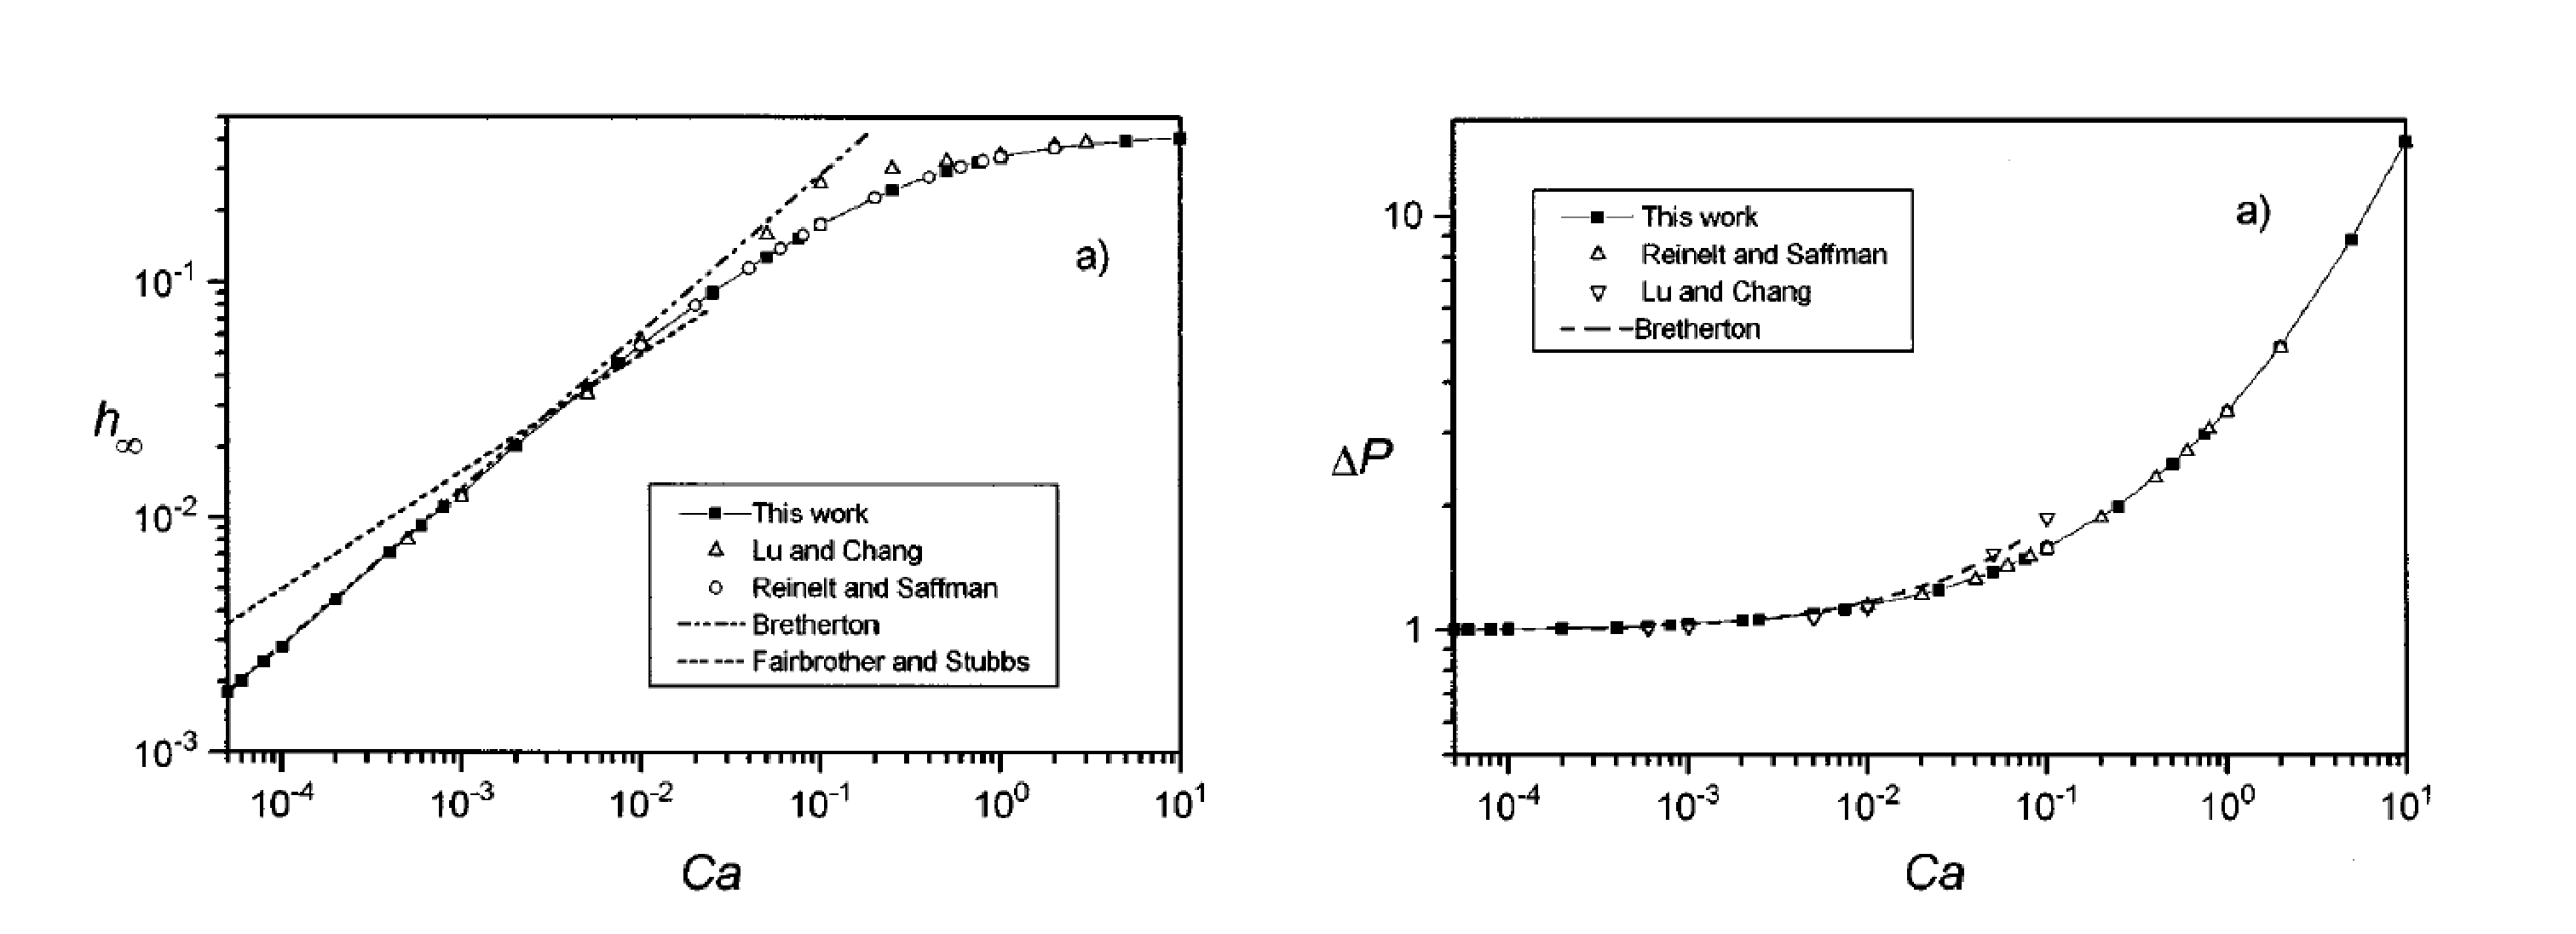
\includegraphics[width=0.97\textwidth]{Figures/giavedoni_planar.eps}
\caption{\citet{giavedoni-numerical} gathered results across the
literature for different Capillary numbers \label{fig:giavedoni:planar}}
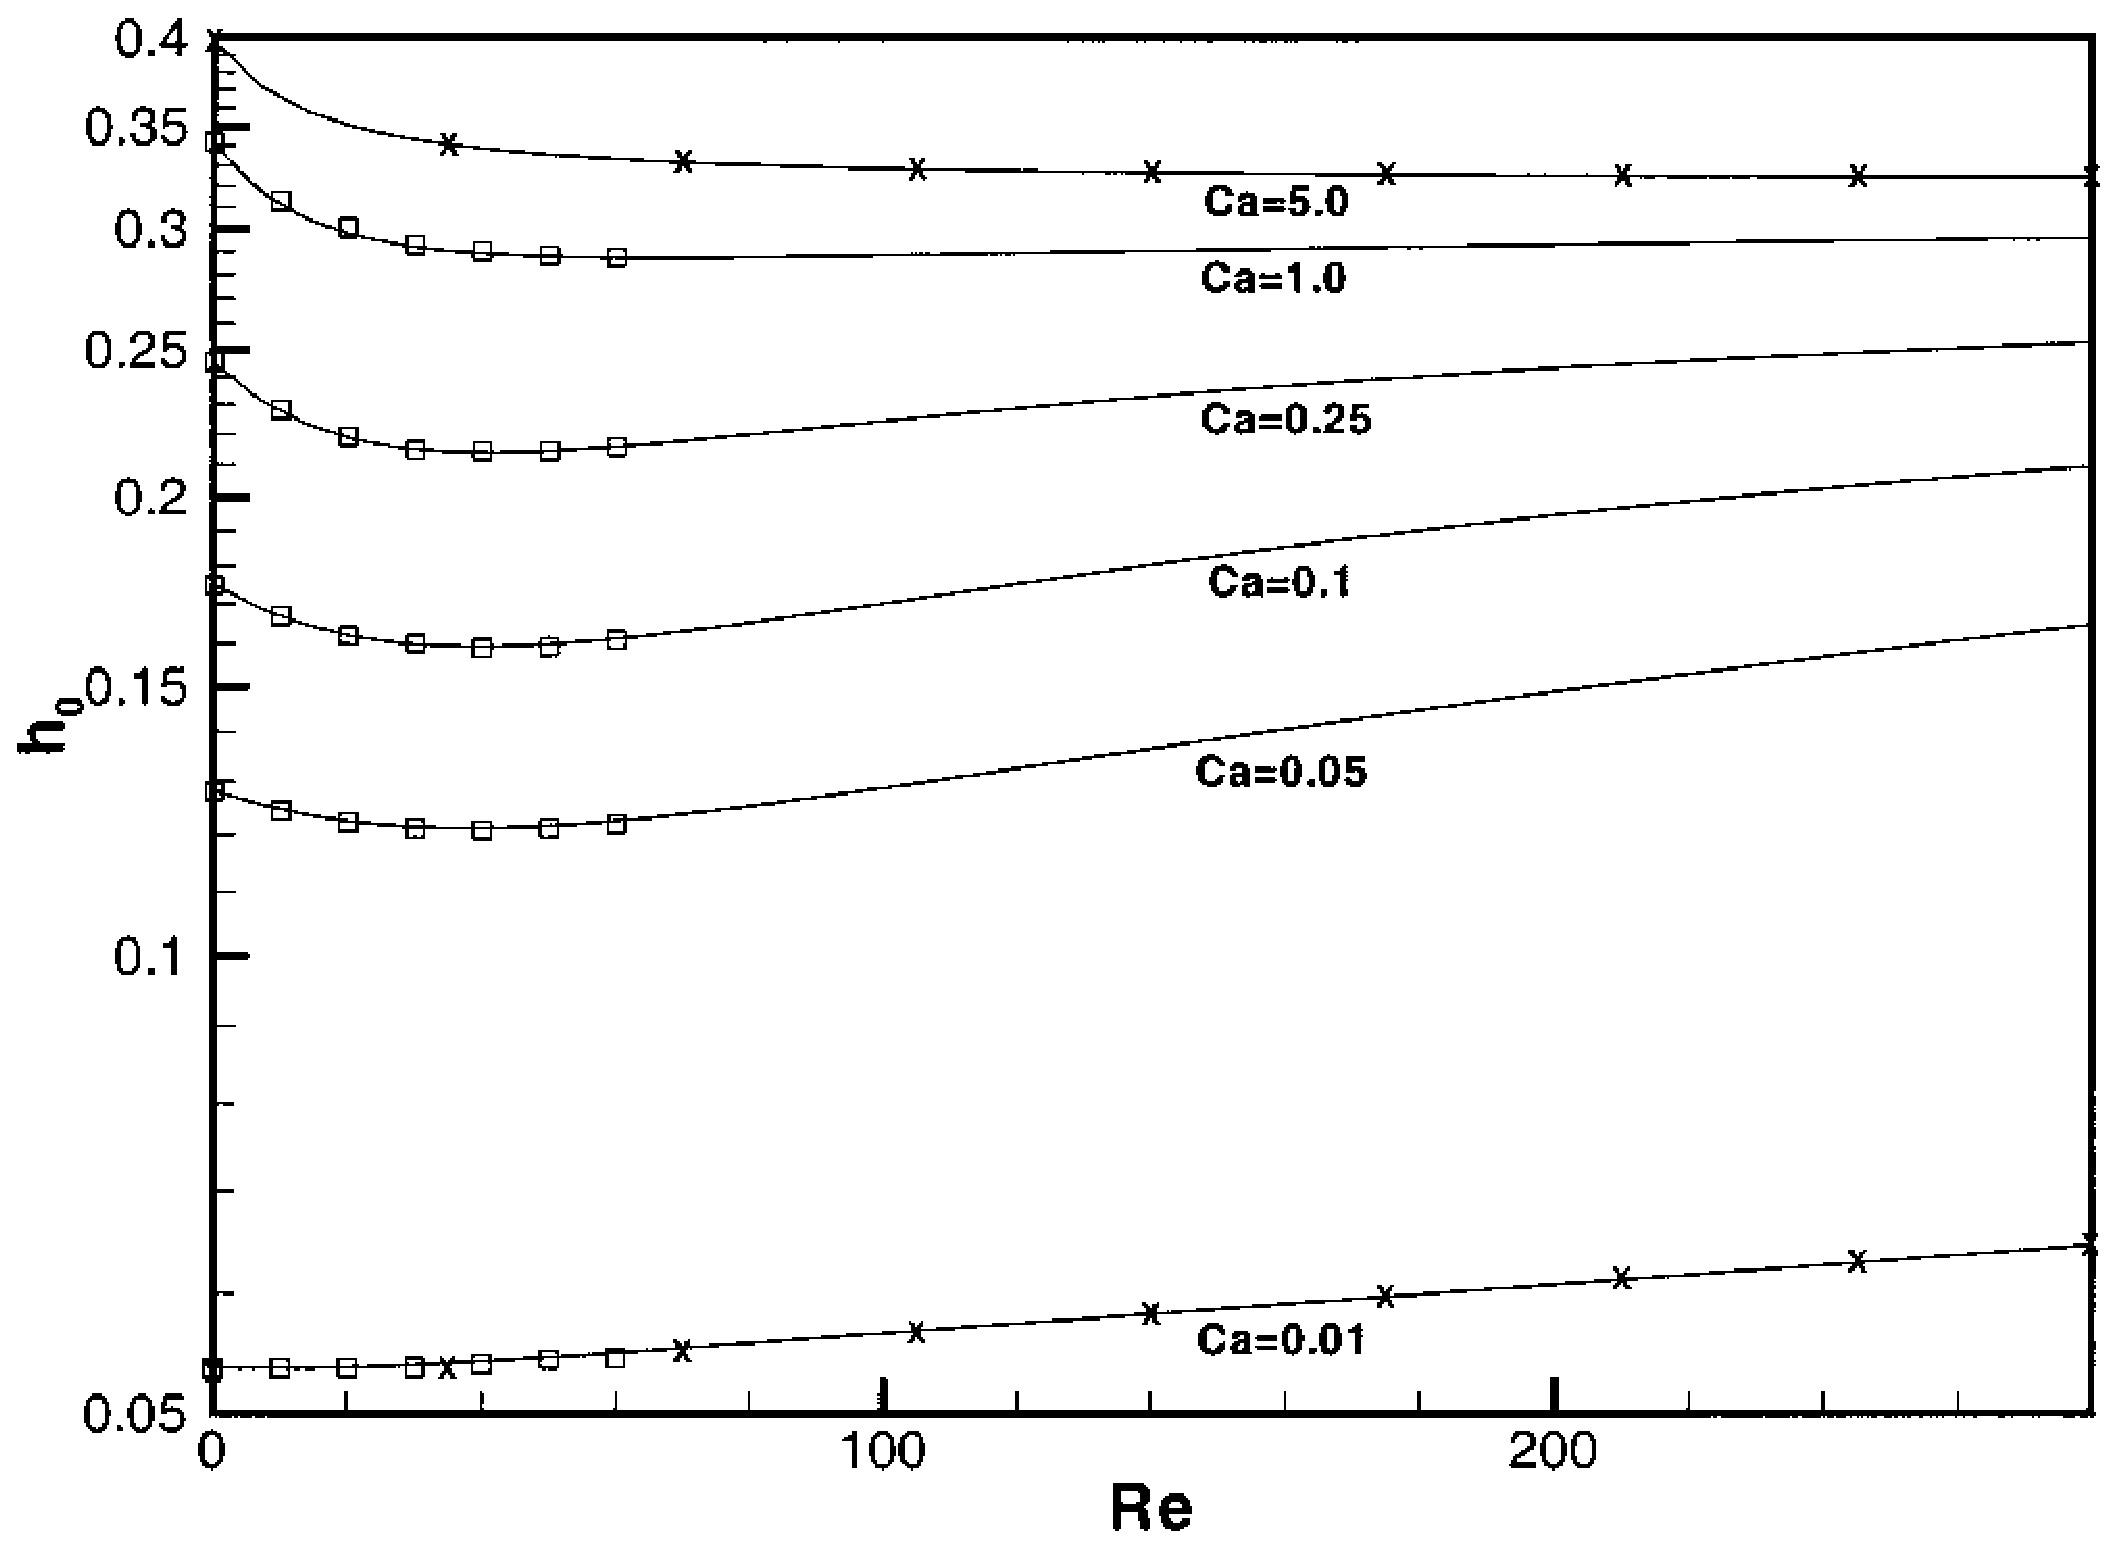
\includegraphics[width=0.97\textwidth]{Figures/heil-planar.eps}
\caption{\citet{heil-bretherton} performed simulations for different ranges of
Capillary numbers and Reynolds numbers. \label{fig:heil:planar}}
\end{figure}
Note that we base the initialization techniques through correlations for the
capillary number and the body force. However, in the binary liquid framework
those correlations give only the approximation. First of all the body force
which is based on the Poiesuille velocity profile for the liquid phase is the
biggest assumption. In reality the less viscous bubble will have a slippage
factor and its velocity is larger than the surrounding liquid velocity. By
plugging in the obtained velocity back to the capillary number equation the
larger capillary number can be obtained. While we present the initialization
tips, in reality one needs to take the bubble velocity from the simulations and
recalculate all the necessary characteristics or in other words adjust the
forcing to obtain the desired velocity/capillary number. 

\subsection{Grid refinement}
To properly estimate the interface resolution one needs to perform the
convergence study dependance on the grid resolution. All parameters are fixed,
including a bubble velocity, the capillary number and change the grid
resolution. Our goal is to know exactly the ratio of the interface width to the
film thickness where results are not dependant on the grid resolution. 

The example what we want to simulate is the capillary number
$0.05$. As it was pointed out the film thickness in that case is $6$ percent.
Note that in the case of half-way bounce-back walls which are used in the
simulations one needs to calculate the film thickness as: 
\begin{equation}
\delta=(\phi_0-0.5)/(N_y-2),
\end{equation}
where $\phi_0$ is the grid coordinate where phase field equals to $0$, $N_y-2$
is related to the effective channel height. Note that it's a big
simplifications to impose the boundary in the middle beetween the bounce-back
node and the fluid node. In the case of $\delta=0.06$ the initial grid number
is $N_y=102$, which gives the horizontal grid number as $N_x-1=15(N_y-2)=1500$.
The bubble is initialized as rectangular box with coordinates
$y=7\dots N_y-8$, $x=\frac{N_x}{3}\dots \frac{2 N_x}{3}$ and phase
$\phi_{bubble}=-1$. All other nodes are initialized with the phase field
$\phi=1$. The force gradient can be estimated through the Poiseuille
profile formula, Eq.\ref{poiseuille:velocity:center}, and it equals
$1.508\,10^{-6}$.

After choosing the reference parameters, the grid refinement needs to keep the
same the same macroscopic parameters as capillary number and viscosities ratio.
Therefore the simulations were performed with grid
numbers $N_y=102,127,152,177,202,227$, corresponding to the
effective channels widths as $H_{eff}=100,125,150,175,200,225$,
$N_x=1501,1876,2251,2626,3001,3376=15
H_{eff}+1$. It is easy to check
that keeping all liquid viscosities the same yields the following quantity to
be a
constant while doing the grid refinement
$H_{eff}^2\frac{\mathrm{d}P}{\mathrm{d}x}=(N_y-2)^2\frac{\mathrm{d}P}{\mathrm{d}
x } =Const$.
{\color{red} Michal, please add some results here and description to it as well.
The results for the force driven flows velocity phase profiles are shown in
Fig. \ref{fig:grid:profiles}. The corresponding ratios to the effective channel
width (without bounce-back nodes) is as $0.0809472165313,
0.0708111118485, 0.0678483852412, 0.0664499716904$. One can see
that for the channel widths as $149,198$, the results are convergent. The
velocities in the center of the bubble are $0.004176469553,
0.00401004133, 0.003969909065, 0.00394134433$, which corresponds
to the $Ca=\frac{\mu_{liq} U_{bubble}}{\gamma}=\frac{\frac{2}{3}\,
0.0045}{0.03771}=0.069$, which is slightly higher when for the assumed
profile. However, if we define Capillary number through the velocity of the
slug, then the Capillary number will have another value. The velocities of the
slug are $0.003411444831,0.003412693869,0.003420338754,0.003425757312$ and
Capillary number defined through these velocities is $0.0602$. 
}
Let us calculate to which extent we need to refine the interface to obtain
convergent results. The interface itself occupies approximately $5 \xi$, where
$\xi=\sqrt{k/A}=1$. This interface width divided to the effective channel width
($5\xi/H_{eff}$) is as follows {\color{red} Please add new values here
$0.102,0.051,0.034,0.025$ } for the given
$H_{eff}$. Let us calculate the interface width ratio to the film thickness as
$5\xi/H_{film}$ is as follows
{\color{red} Please add here new values $1.2605,  0.7205,  0.501,  0.3839$}.
Therefore, one needs to
resolve the interface as {\color{red} Please give number here $40\%$} of the
expected film width for simulations to be converged.
{\color{red} If we need this pictures???
\begin{figure}
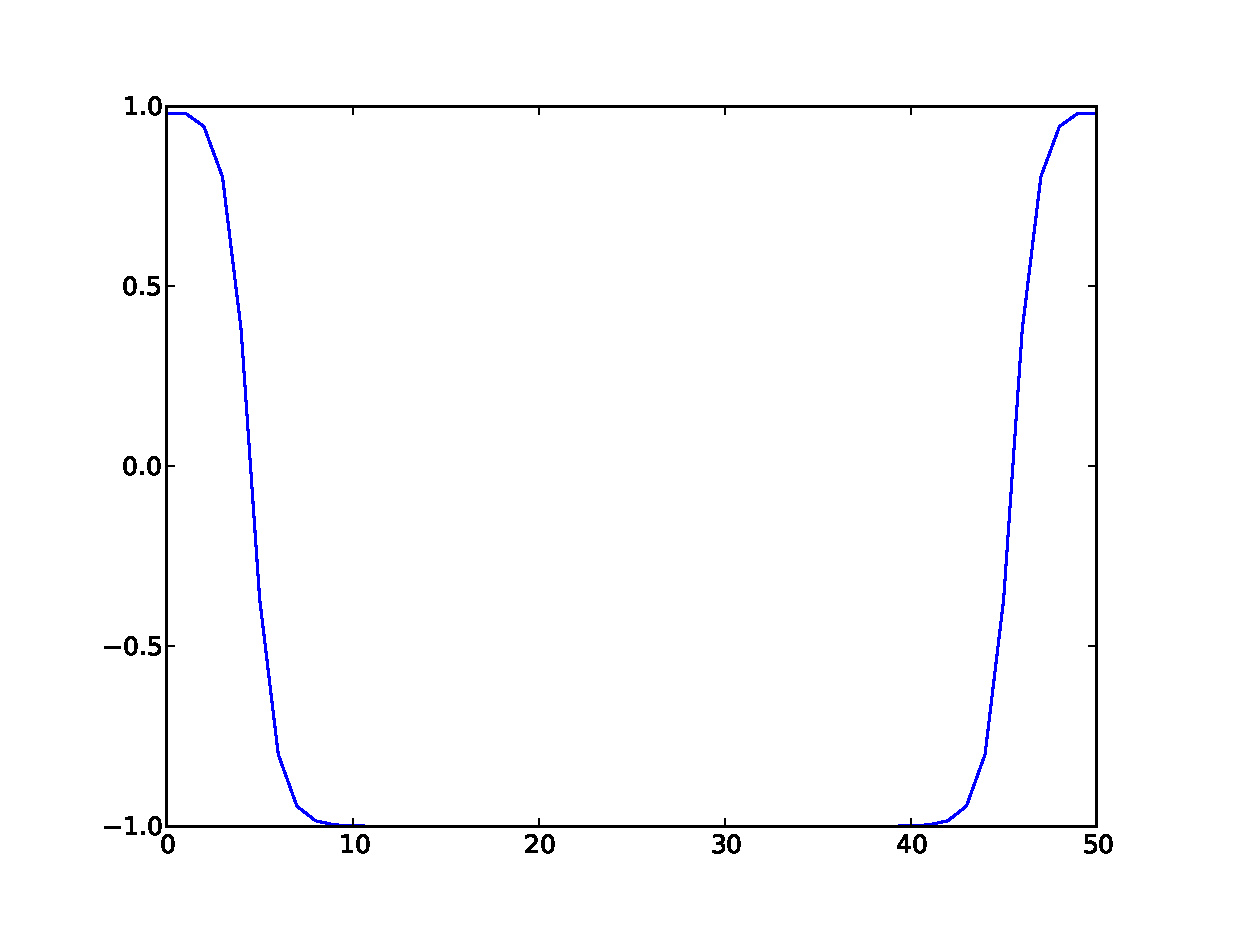
\includegraphics[width=0.47\textwidth]{Figures/grid_phase_prof_49.eps}\hfill
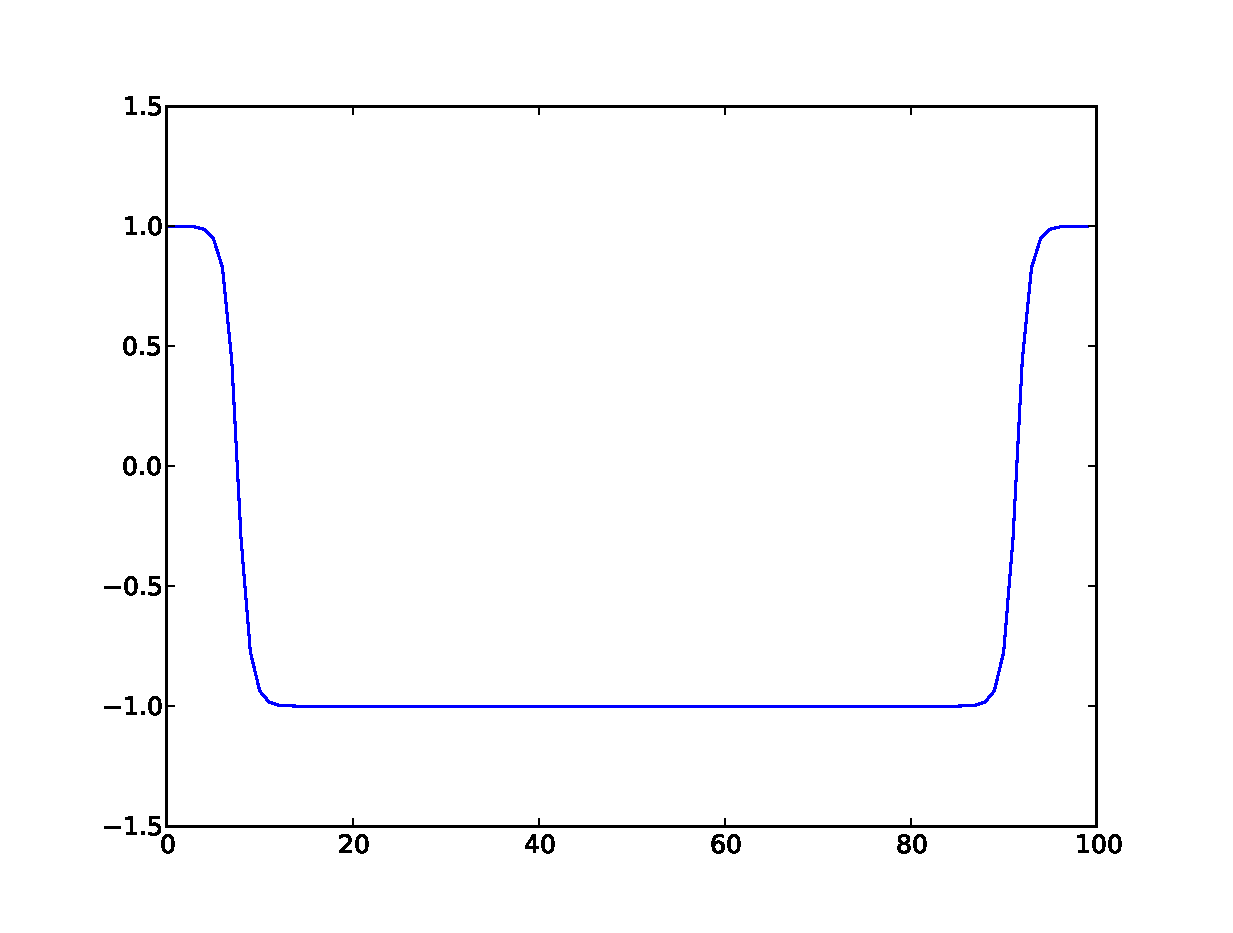
\includegraphics[width=0.47\textwidth]{Figures/grid_phase_prof_98.eps}\\
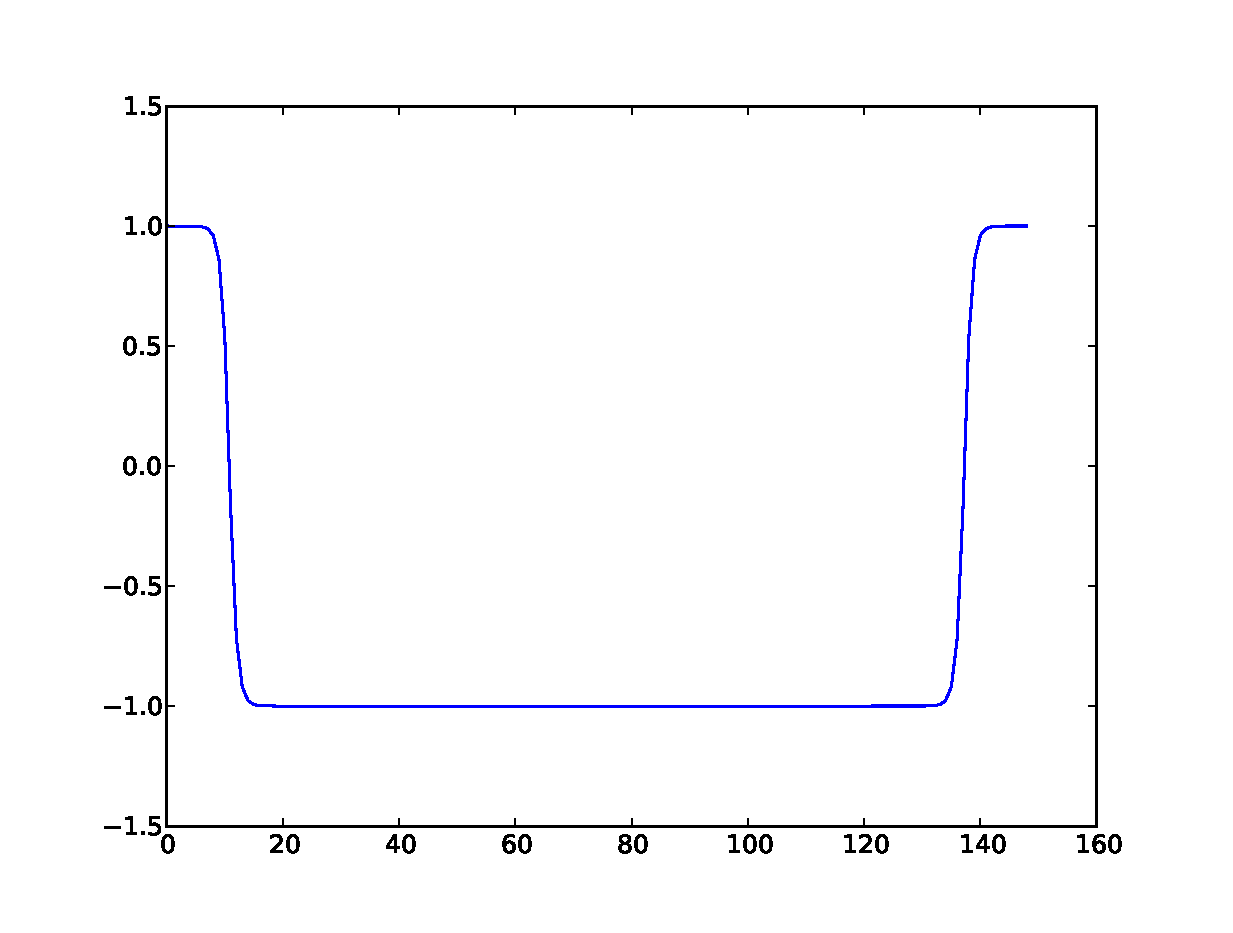
\includegraphics[width=0.47\textwidth]{Figures/grid_phase_prof_147.eps}\hfill
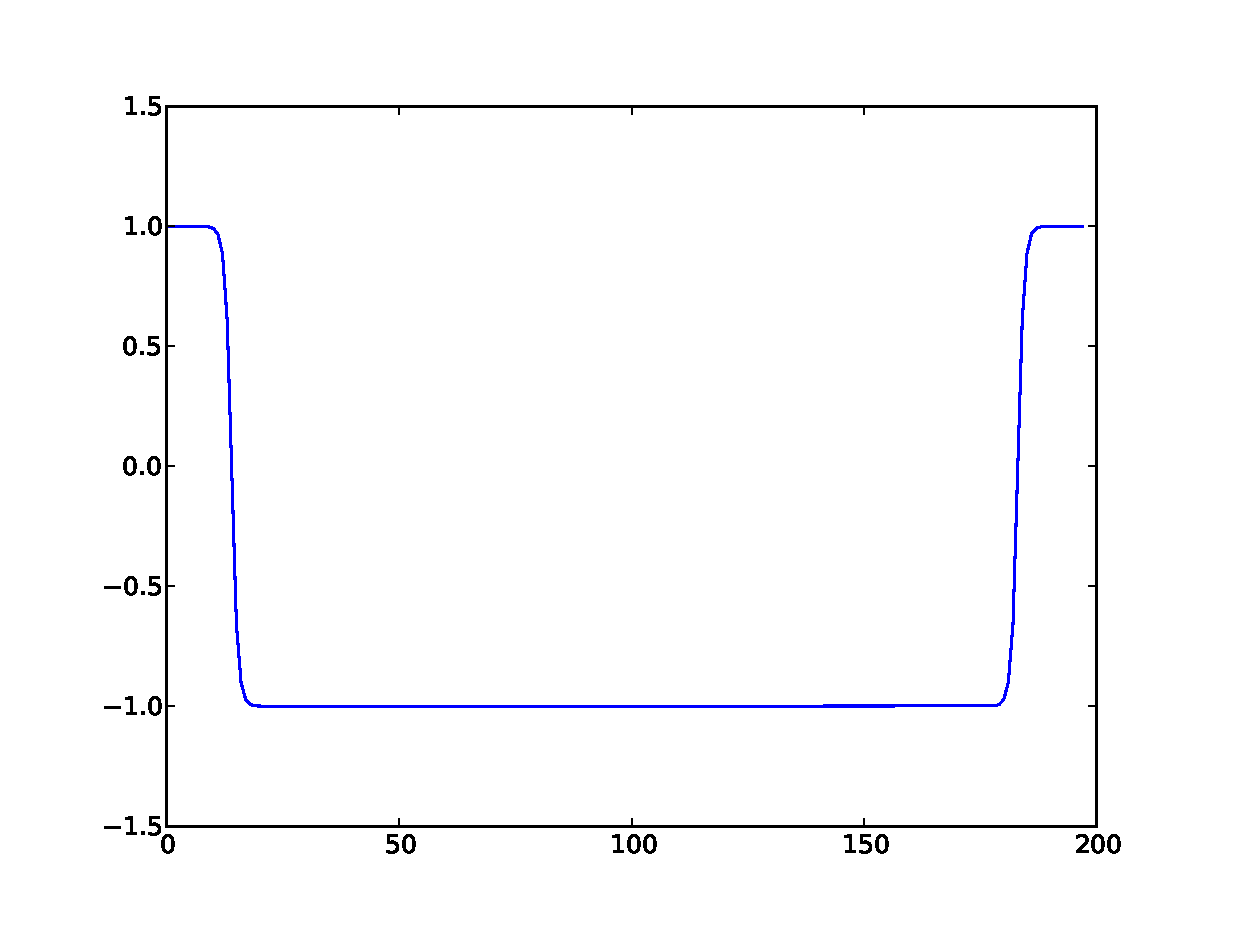
\includegraphics[width=0.47\textwidth]{Figures/grid_phase_prof_196.eps}\\
\caption{Do we need these pictures? Grid refined profiles for the effictive
channel widths
$H_{eff}=49,98,147,196$.\label{fig:grid:profiles}}
\end{figure}
}

\subsection{The influence of the wall gradient}
Once the procedure of how to resolve the interface gradient is known, we want
to examine the influence of the phase gradient, i.e. the wettability of the
wall, to the film thickness. We examined the
wall gradient influence on
the standard grid $202\mathrm{x}3001$ and the initial film width as
{\color{red} Take the value from previous calculations $20$}
lattice boltzmann units. We examined $11$ different values for the wall
gradient ranging from $-1$ to $1$. The results are consistent among all the
wall gradients given that the interface is resolved in the right way. For the
given wall gradients the values of interface thicknesses are
{\color{red} Change these numbers $0.0709130255276, 0.0708903443305,
0.0708661222722,
0.0708369188112, 0.0707962325316, 0.0707266326981, 0.0705839443249,
0.0702489349415, 0.0697553433989$}. For the wall gradients $0.8$ and $1.0$ the
values are NAN. The negative values of the phase gradient are preferable, as
far as the phase of the liquid adjacent to the wall has the value of $1$. That
means that the phase values near the wall are above $1$. In case of positive
gradients the values near the wall are below $1$ and the gradient profile can
fuse with the values of the gas phase as $-1$, creating the wall stickyness,
unphysical one. {\color{red} Michal, if you want to add some pictures go ahead
with it}.

\section{The influence of different viscosities}
The results obtained earlier are taken for the liquiqs viscosity ratio $10$.
We performed the same simulations for the liquids viscosity ratio as $20$.
Parameters were taken as $\tau_{liquid}=4.5$ and $\tau_{bubble}=0.7$. 
{\color{red} The results showed that blah-blah-blah - I guess will be the same}.

\section{Capillary number region}
The purpose of this section is to validate the correlations of
\citet{giavedoni-numerical}, Fig. \ref{fig:giavedoni:planar}, and
\citet{heil-bretherton}, Fig. \ref{fig:heil:planar}, for the range of capillary
numbers. Because of limiting computational factors ({\color{red} What is the
least capillary number which is OK?}) we cannot go to the range of small
capillary numbers. However, all the other methods were validated across the
small capilary numbers and extended for the range of capillary numbers from
$0.005$ to $1.0$. Our goal is to compare the film thickness over the capillary
range from $0.03$ to $1.0$. 

To perform numerical simulations we refer to
grid refinement section where we obtained that the interface width should be
at most {\color{red} $40$} percent of the interface width. For the benchmark
results we
suggest the following Capillary numbers as:
\begin{equation}
0.03,0.05,0.08,0.1,0.2,0.4,0.6,0.8,1.0\, .
\end{equation}
The corresponding approximate film widths from \cite{giavedoni-numerical} are as
follows:
$0.04,0.06,0.08,0.1,0.12,0.13,0.15$. $5$ lattice boltzmann units occupy
{\color{red} Could be another number $40\%$} of the interface thickness.
Therefore the grid size should be as
following {\color{red} Michal, different numbers would be here.
$314\mathrm{x}4681$,$210\mathrm{x}3121$,
$158\mathrm{x}2341$, $127\mathrm{x}1876$, $106\mathrm{x}1561$,
$98\mathrm{x}1441$,$85\mathrm{x}1246$ Michal, for the larger capillary
numbers such small grid is not
appropriate because of the instabilities.
}.

{\color{red} Probably we don't need the explanations about initialization here,
just to present results}
To utilize previous results to properly initialize simulations to run one need
to do some modifications. The result is that for the grid with $H_{eff}=200$ we
obtained the film width as {\color{red} Will be another number $0.0685$} and
velocity in the center of the bubble as
{\color{red} Will be another number $0.0045$}. The force gradient was
{\color{red} Probably the same number $6\, 10^{-6} /16$}. The predicted
Capillary
number was $0.05$ and the actual one based on the center velocity calculation is
{\color{red} Will be another number $0.0795$}. However, we performed simulations
according the assumed value of $0.05$. Let us perform some correlations to
calculate how the system needs to be initialized. 
\begin{equation}
\begin{aligned}
&Ca_{lit} \propto U_{slug}\\
&U_{slug} \propto \frac{\mathrm{d}P}{\mathrm{d}x} N_y^2\\ 
&Ca_{lit} \propto \frac{\mathrm{d}P}{\mathrm{d} x} N_y^2 \text{ or }\\
&\frac{\mathrm{d}P}{\mathrm{d} x} \propto \frac{Ca_{lit}}{Ny^2},
\end{aligned}
\end{equation}
where the index $lit$ stands for the presented in the literature in
\cite{giavedoni-numerical,heil-bretherton}. Therefore the initialized consistent
pressure gradients can be taken from
previous consistent simulations:
\begin{equation}
\frac{\mathrm{d}P}{\mathrm{d} x}=6\,10^{-6}/16 \frac{Ca_{literature}}{0.05}
\frac{200^2}{N_y^2}=0.3 \frac{Ca_{literature}}{N_y^2}
\end{equation}
Note that $N_y$ is calculated through the expected resolution of the interface
in comparison with the interface thickness which itself is based on
Capillary number simulations. In terms of time the steady state successful
simulation for the grid $202\mathrm{x}3001$ was obtained after $200,000$ steps.
The physical
time is as follows:
\begin{equation}
\begin{aligned}
&\Delta t=\frac{U_{slug,LB} \Delta X}{U_{phys}} \propto \frac{1}{N_y-2}\\
&N_{iter}=200,000 \frac{N_y-2}{200}\approx 1000 N_y\\
%&N_{output}=51 Ny\\
\end{aligned}
\end{equation}

{\color{red} That's why we need better grid for larger Capillary numbers. Steady
simulations were obtained for the following Capillary numbers
$0.03,0.05,0.08,0.1$  }with the film thicknesses as
{\color{red} $0.0337433850478, 0.063192148642, 0.0799078589211,
0.0891674460655$} which are
quite close to the predicted one $0.04,0.06,0.08,0.1$. The thing is to identify
the Capillary numbers associated with those numbers. The velocity in the
centers are $0.00209258774,0.003826643811,0.006506324324,0.008333889077$. The
Capillary numbers associated with these velocities are $0.036992074529545796, 
0.067646144698590829,0.1150166512524845,0.14732373700007995$, which again a bit
overpredictive but consistent. The fig.
\ref{fig:capillary:simple} represents the thickness against the Capillary
number which mimics the curve behavior for the Capillary number dependance as
indicated in Fig. \ref{fig:giavedoni:planar}.
\begin{figure}
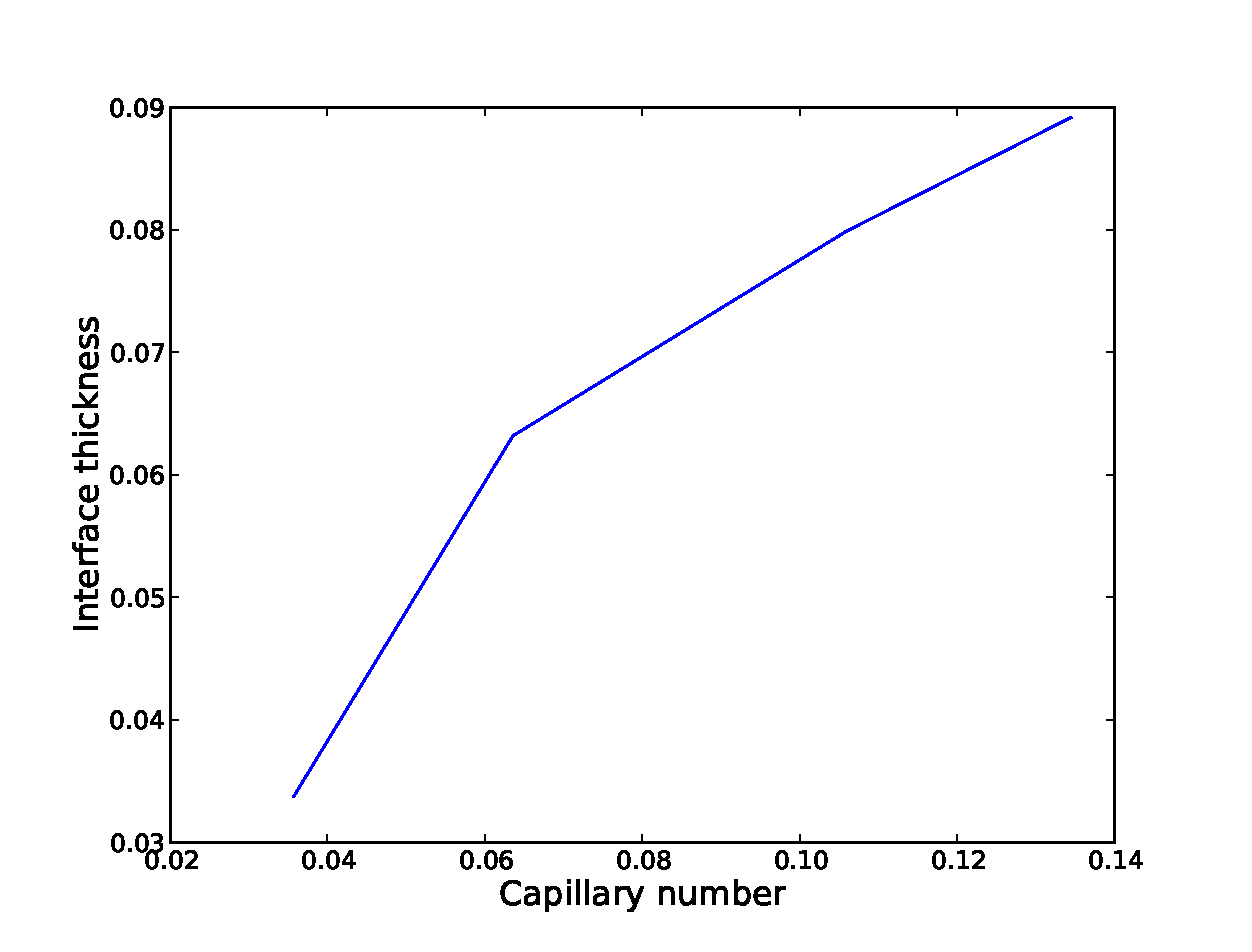
\includegraphics[width=0.47\textwidth]{Figures/capillary_thickness_simple.eps}
\hfill
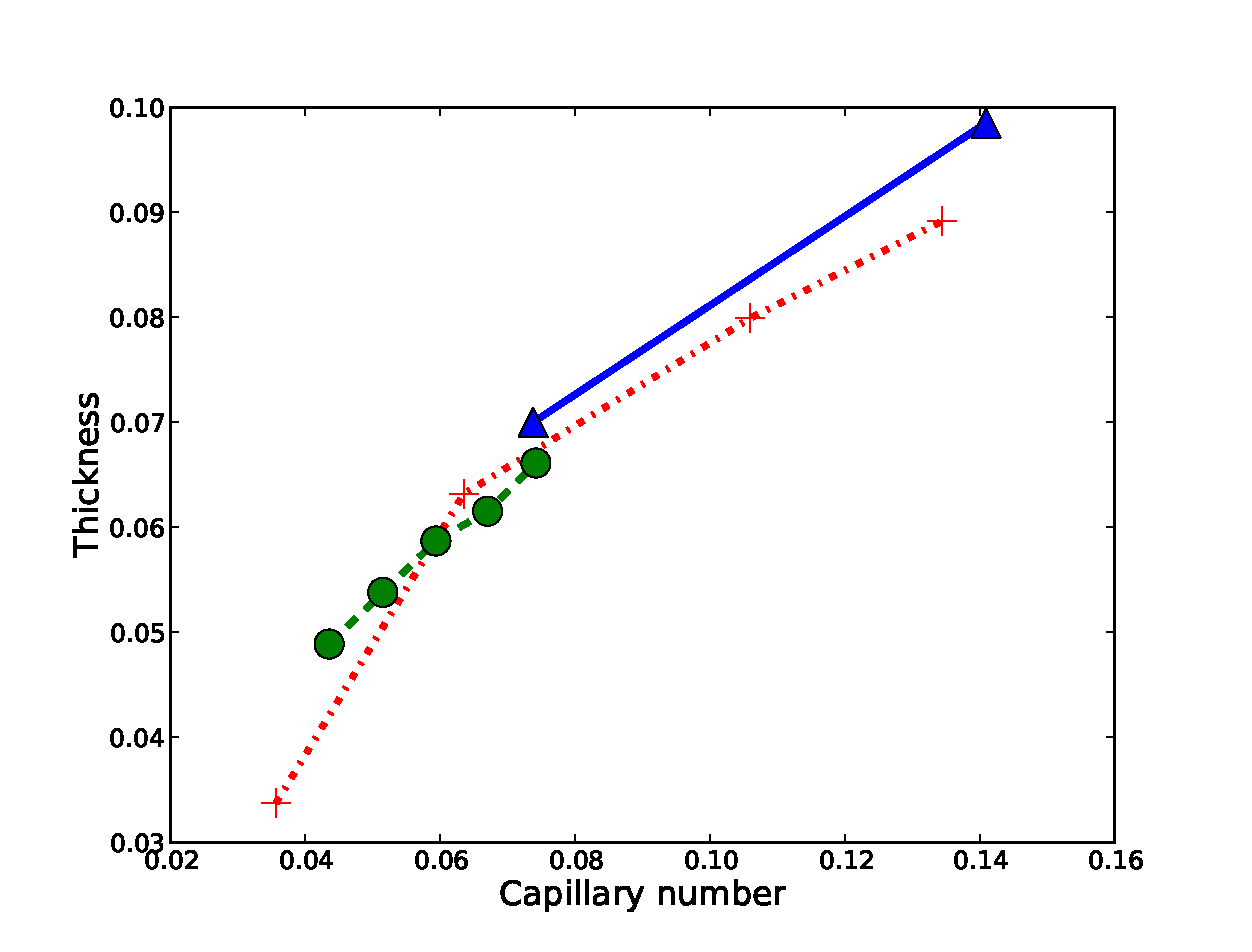
\includegraphics[width=0.47\textwidth]{Figures/capillary_range.eps}
\caption{{\color{red} This one to eliminate - just present here
comparison between our simulations in the longer range of capillary
numbers and Giavedoni}Thickness versus the capillary
number for different scalings based on
the average capillary number. \label{fig:capillary:simple}}
\end{figure}

\subsection{The influence of the force}

{\color{red} Michal if you find it useful - use this section. My suggestion is
to eliminate it.}
\begin{description}
 \item 
On the grid $198\mathrm{x}2941$ and the initial film width as $20$ units
the
influence of the force is studied. $16$ different values of force are examined,
which have the following expression $\frac{0.000006}{16} i$, where $i=1 \dots
16$. The system is allowed to come to the equilibrium after $200,000$ steps. The
goal is to study the influence of the force on the velocity and therefore the
capillary number. Unfortunately in the first case only a few simulations are
stable, i.e.
$i=1,2$ is stable. The results for the interface thicknesses are
$0.0700122222668,0.0985152303286$ with the velocities associated as
$0.004490013864,0.009597299475$. Those numbers correspond to the bubble
capillary numbers as $0.079372981271400328, 0.16965788849626481$. The average
capillary numbers are $0.07381636,0.14095644$. 

\item
On the grid $394\mathrm{x}5881$ and the initial film width as $20+4 i$,where
$i=1 \dots 5$ units the
influence of the force is studied. The force is scheduled as
$\frac{0.000006}{128}+i \frac{0.000006}{640}$.The intention is to cover the
calculation of the Capillary numbers in the range $0.03,0.035,0.04,0.045,0.05$. 
$5$ different values of force are examined. The system is allowed to come to the
equilibrium after $400,000-40,000 i$ steps. The associated thicknesses were as
it follows
$0.0488915027016,0.0538098132568,0.0587100833678,0.0615470184196,
0.0661331899123$. Bubble velocities are
$0.002592856205,0.003077834398,0.003562975124,0.004034533823,0.004470657603$.
Bubble Capillary numbers are $0.04583566,  0.05440894,  0.0629851 , 
0.07132116, 0.07903081$.
\end{description}

\section{Conclusion}
The work presents the numerical tips and the benchmark for the
Bretherton/Taylor problem using the binary liquid lattice Botlzmann method. The
results show consistency with the already obtained numerical correlations using
other methods. Though results are specific for the binary liquid lattice
Botlzmann method but numerical tips and correlations can be used for any
continuous interface methods. The work is valuable for people simulating
microchannel flows.

\bibliographystyle{plainnat}
\bibliography{paper}

\end{document}
